\documentclass{article}
\usepackage[T1]{fontenc}
\usepackage[utf8]{inputenc}
\usepackage[a4paper, total={6in, 8in}]{geometry}
%\usepackage[icelandic]{babel}
\usepackage{graphicx} %package to manage images


\usepackage{xcolor}
\usepackage{listings}

\colorlet{mygray}{black!30}
\colorlet{mygreen}{green!60!blue}
\colorlet{mymauve}{red!60!blue}

\lstset{
  backgroundcolor=\color{gray!10},  
  basicstyle=\ttfamily,
  columns=fullflexible,
  breakatwhitespace=false,      
  breaklines=true,                
  captionpos=b,                    
  commentstyle=\color{mygreen}, 
  extendedchars=true,              
  frame=single,                   
  keepspaces=true,             
  keywordstyle=\color{blue},      
  language=c++,                 
  numbers=none,                
  numbersep=5pt,                   
  numberstyle=\tiny\color{blue}, 
  rulecolor=\color{mygray},        
  showspaces=false,               
  showtabs=false,                 
  stepnumber=5,                  
  stringstyle=\color{mymauve},    
  tabsize=3,                                     
  title=\lstname 
}

\title{Embedded Group Project}
\author{Steinarr Hrafn Höskuldsson\\
Arnþór Gíslason\\
Reykjavik University}
\date{September 2022}

\begin{document}

\maketitle

\section*{Part 1}
The hall effect sensor has 7 hole pairs and with each revolution of the motor shaft the signal will cycle 7 times. With two signals, 90° out of phase there are 28 edges per revolution equally spaced. The maximum motor speed is rated at 15.000 RPM or 250 Hz. The minimum time between edges is thus expected to be \((28*250Hz)^{-1}) = 143 \mu s\)

We wrote an encoder class that polls pins 9 and 10 on the Arduino and keeps track of how many pulses have been registered. 

We wired the two signals and the signal from the LED pin to an RTB2004 oscilloscope and observed that we could turn the LED on for 120 microseconds without dropping pulses. 


However, printing the result to the serial port at 9600 baud takes around a millisecond per character. Thus we are dropping pulses while writing to the serial port.


With the motor running, a pin was toggled each time the monitor detected a state change. A jitter and a period of inactivity on the toggled pin was observed indicating that there were periods where the microcontroller was missing pulses while transmitting on the UART. The baud rade was set at 9600 baud which translates to about 1ms per character written and th

\begin{figure}[h]
    \centering
    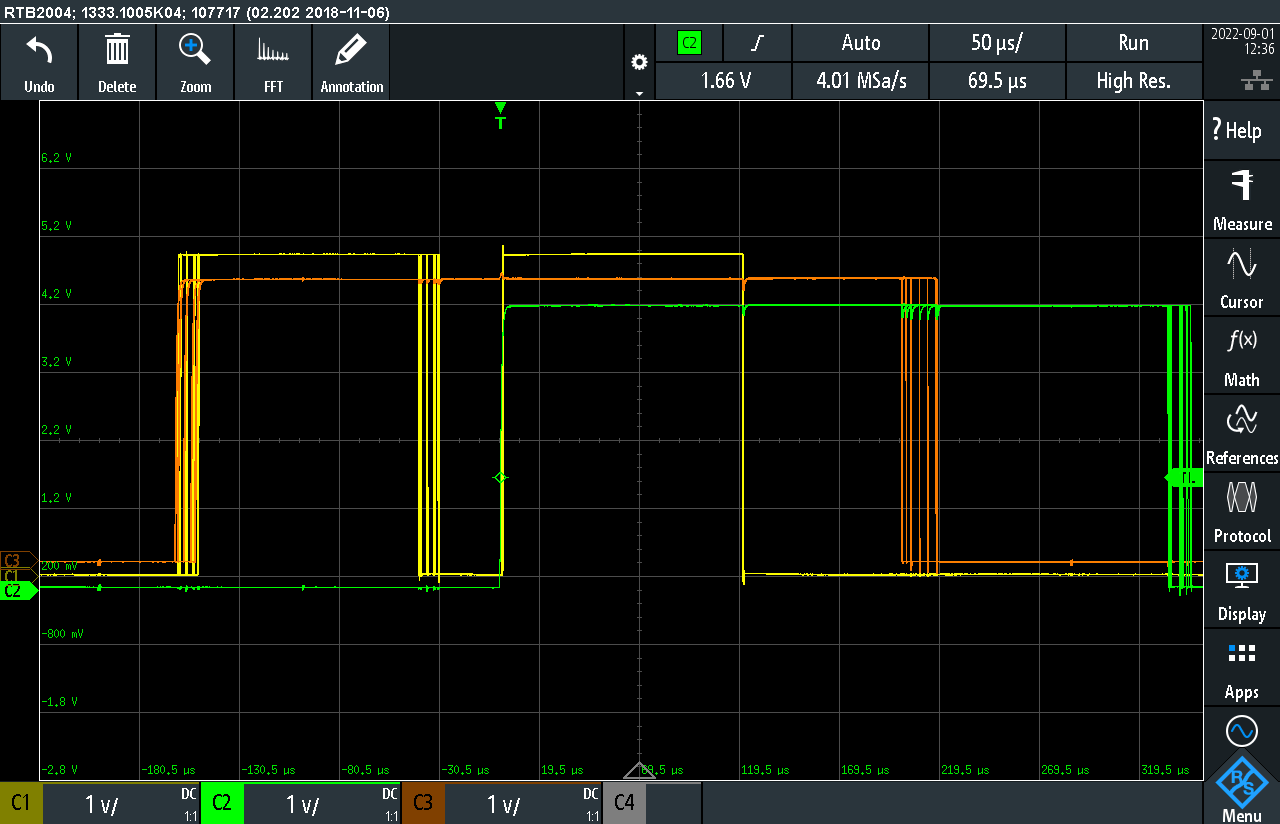
\includegraphics[width=0.75\textwidth]{Project1RotaryEncoder/oscilloscope_part1_120ms.PNG}
    \caption{Screenshot of the RTB2004 oscilloscope, LED (yellow) is turned on for 120 microsecond at pulse detection. Note that the graphs have been vertically shifted slightly to make them more visible.}
    \label{fig:osc120}
\end{figure}

\begin{figure}[h]
    \centering
    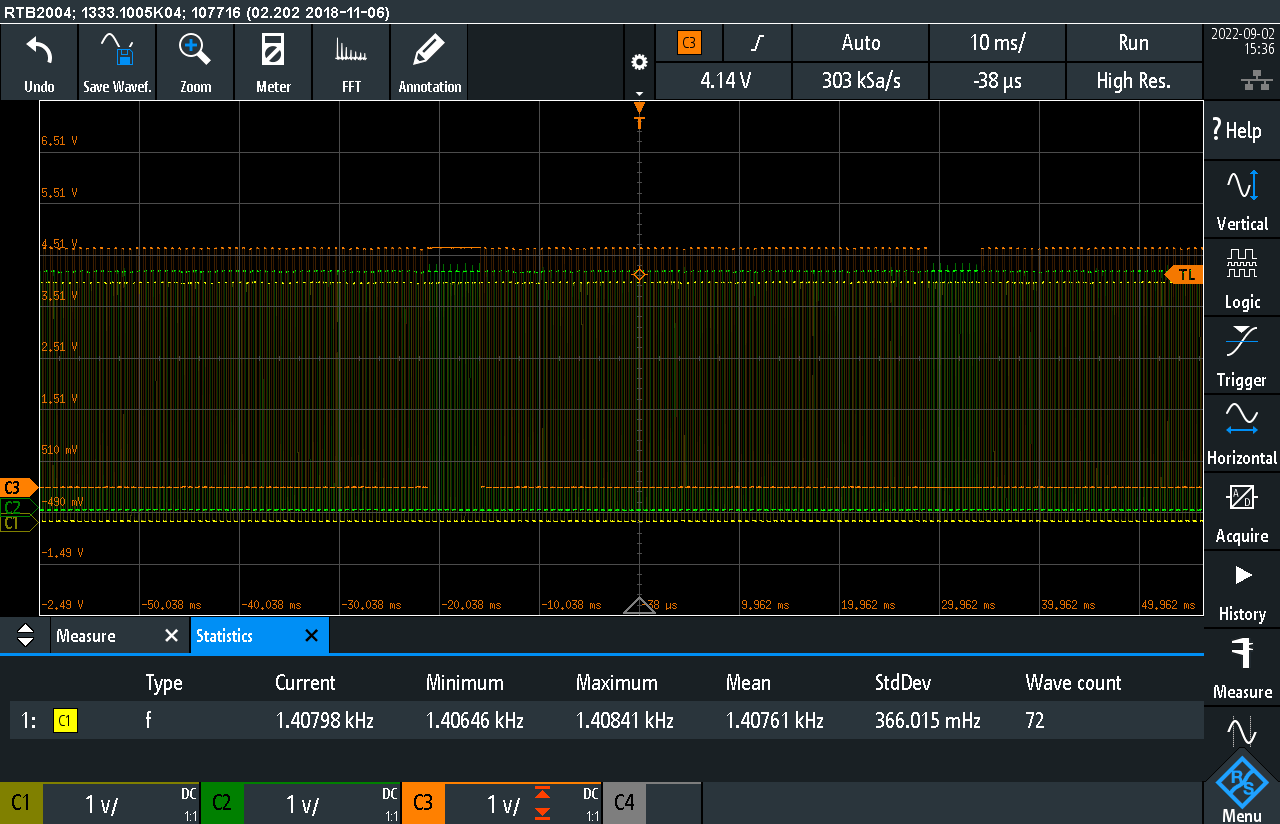
\includegraphics[width=0.75\textwidth]{Project1RotaryEncoder/oscilloscope_missing_pulses.PNG}
    \caption{While writing to the serial port, the Arduino is not polling the input pins, causing dropped pulses. This can be seen in the missing LED(orange) pulses}
    \label{fig:oscdrop}
\end{figure}


\section*{Part 2}
Using interrupts to monitor the pins allows us to count the pulses even while writing to the serial port.


\appendix
\section{Code}\label{appendix:code}

\lstinputlisting[caption=encoder\_simple.h]{Project1RotaryEncoder/src/encoder_simple.h}

\lstinputlisting[caption=timer\_msec.cpp]{Project1RotaryEncoder/src/encoder_simple.cpp}

\lstinputlisting[caption=main.cpp]{Project1RotaryEncoder/src/main.cpp}

\end{document}
